\documentclass[11pt,usepdftitle=false]{beamer}

% Languages.
\RequirePackage{polyglossia}
\setdefaultlanguage{russian}
\setotherlanguage{english}

% Fonts.
\usepackage{fontspec}
\newfontfamily\russianfontsf[Ligatures=TeX]{Bender}
\newfontfamily\englishfontsf[Ligatures=TeX]{Bender}
\newfontfamily\russianfonttt{Source Code Pro}
\newfontfamily\englishfonttt{Source Code Pro}

\graphicspath{{figures/}}

\usepackage[parfill]{parskip}
\usepackage{booktabs}

%% Custom commands and environments.

\newcommand*{\en}{\textenglish}

\author{Ада Лавлейс\\Научный руководитель: Дональд Кнут}
\title{Симуляция работы протокола физического уровня модели OSI через среду астральной плоскости}
\subtitle{Выпускная квалификационная работа}
%\logo{}
\institute{Казанский Федеральный Университет\\Высшая Школа Информационных Технологий и Информационных Систем}
\titlegraphic{
\includegraphics[height=3ex]{itis_logo}}
\date{99 декабря 2099 г.}
%\subject{}

\hypersetup{%
    pdftitle=\inserttitle,%
    pdfauthor={Ада Лавлейс},%
    pdfsubject=\insertsubtitle,%
}

\usecolortheme{dove}
%\usefonttheme{structuresmallcapsserif}

%\useoutertheme{infolines}
%\useoutertheme[footline=authortitle]{miniframes}

\setbeamertemplate{navigation symbols}{}
\setbeamertemplate{itemize items}[square]
\setbeamertemplate{enumerate items}[square]

%\setbeamertemplate{footline}[page number]
\setbeamertemplate{footline}[frame number]
%\setbeamertemplate{footline}[infolines theme]
%\setbeamertemplate{footline}[miniframes theme]

%\AtBeginSection[]{%
%    \begin{frame}
%        \frametitle{Table of Contents}
%        \tableofcontents[currentsection]
%    \end{frame}
%}

\AtBeginSection[]{%
    \frame{\centering\Huge\insertsection}%
}

\begin{document}
\frame[plain]\titlepage

\section{Введение}

\subsection{Астральный план}
\begin{frame}\frametitle\insertsubsection
\centering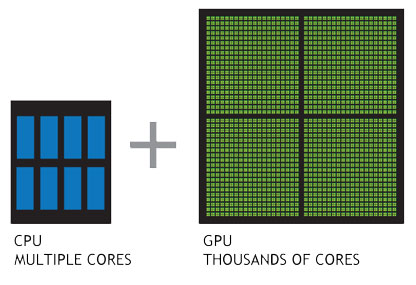
\includegraphics[height=0.5\textheight]{cpu_and_gpu}
\begin{itemize}
\item Интересная тема для исследований
\item Большие возможности для передачи данных
\end{itemize}
\end{frame}

\section{Концепция}

\subsection{Модель OSI}
\begin{frame}\frametitle\insertsubsection
\begin{columns}
\column{0.5\linewidth}
\begin{enumerate}
\item Физический уровень
\item Канальный уровень
\item \dots
\end{enumerate}
\column{0.5\linewidth}
TCP/IP
\end{columns}
\end{frame}

\begin{frame}[plain]
\centering\Huge

Последний слайд

\mbox{}

1--2 ключевых идеи
\end{frame}

\end{document}
